% !TEX root = ../../main.tex
\section{Results}\label{sec:artificial_data_results}
For an objective measure of quality of the proposed method applied to the four aforementioned data sets, we employ two metrics, as defined by Takeuchi \etal \cite{takeuchi2006unifying}.
The first metric is the $\operatorname*{average \_ benefit}$, for which we first need to define the notion of $\operatorname*{benefit}$ for each change:
\begin{equation}\label{eq:benefit}
  \operatorname*{benefit}(y) = 1 - |t_y - t_y^*| / 10  \mbox{~~~(when } |t_y - t_y^*| < 10 \mbox{)},
\end{equation}
where $t_y$ is the time of the discovered change point and $t_y^*$ is the true change time.
We can then define the $\operatorname*{average \_ benefit}$ over all the discovered change points $Y$ as:
\begin{equation}\label{eq:average_benefit}
  \operatorname*{average \_ benefit}(Y) = \frac{\sum_{y=1}^Y \operatorname*{benefit}(y)}{Y}.
\end{equation}
Besides the benefit, which rewards discovered change points close to the actual change points, we need to penalize discovered change points which do not relate to a true change point.
For this we use the \acrlong{far}, expressed as
\begin{equation}\label{eq:false_alarm_rate}
  \operatorname*{far}(Y) = \frac{Y_{\operatorname*{false}}}{Y}.
\end{equation}

For a high quality method the $\operatorname*{average\_benefit}$ should be high and the $\operatorname*{far}$ should be low.

\TODO{Above metrics are not used, remove it and replace with own metric (offset, accuracy)}

The results of all the data sets are provided in \Cref{tab:results_artificial}, together with the used parameters.
For each data set it shows the high and low thresholds used in the \gls{rt} based change detection method.
During the post-processing all detected change points within a certain \emph{closeness} range are merged, for which the value differs per data set.
The difference between the actual and final detected change points are expressed as an offset.
The data sets were processed with different window lengths and $\sigma$ value for the \gls{rbf} kernel.

To give a better impression of the spread of the accuracy of the detected change points, a box plot for each data set is displayed in \Cref{fig:boxplot_artificial_sets}.
With each data set embodying different characteristics, different observations can be drawn from the data sets.
In the references figures, the blue lines represent the radius of the constructed hypersphere.
The vertical red lines are the discovered change points.
For each data set the following is observed:
\begin{enumerate}
  \item \textbf{Fixed increasing mean:} In \Cref{fig:camci_fixed_increasing_mean_thresholds} we see that each change point is almost equally fast and accurate detected.
  This implies that the relative difference between the means of the Gaussian distribution has no effect on the detectability of the algorithm.
  \item \textbf{Reduced increasing mean:} \Cref{fig:takeuchi_reduced_increasing_mean_thresholds} shows that the absolute difference between the means of the Gaussian distribution is a certrain influence to the detectability.
  Although all change points are correctly detected (at the beginning of the series are two outliers), the change in radius becomes less significant at every change point.
  \item \textbf{Reduced increasing mean, increasing variance:} In \Cref{fig:camci_takeuchi_alternating_variance_thresholds} we see the same effect, in regard to the mean, as with the previous data set.
  Furthermore, the increasing variance makes change detection harder.
  This is visible around the $9000$\textsuperscript{th} data point and after, where the radius keeps increasing.
  \item \textbf{Alternating variance:} The ability to detect decreases in variance of the Gaussian distribution is displayed in \Cref{fig:camci_reduced_increasing_mean_increasing_variance_thresholds}.
  Although some change points are discovered with a delay almost up to the length of the window processing the data, the decreases are all detected.
  The box plot of this set, number 4 in \Cref{fig:boxplot_artificial_sets}, shows a wider spread for the results.
\end{enumerate}


\begin{table}
  \centering
  \begin{tabulary}{\textwidth}{|l|c|c|c|c|}
    \cline{2-5}
    \multicolumn{1}{l|}{} & Set 1 & Set 2 & Set 3 & Set 4 \\
    \hline
    High threshold & 1.6 & 1.6 & 1.5 & 2.2 \\
    \hline
    Low threshold & 0.1 & 0.1 & 0.5 & 0.1 \\
    \hline
    Closeness merging & 10 & 10 & 10 & 50 \\
    \hline
    Number of change points detected & 10 & 11 & 11 & 11 \\
    \hline
    Mean offset & 2.27 & 6.18 & 0.64 & 15.36 \\
    \hline
    Standard deviation offset & 1.19 & 7.94 & 0.92 & 17.70 \\
    \hline
    Window length & 50 & 100 & 50 & 50 \\
    \hline
    Sigma of \gls{rbf} & 13 & 13 & 15 & 13 \\
    \hline
  \end{tabulary}
  \caption[Results artificial data sets]{Results of the artificial data sets.}
  \label{tab:results_artificial}
\end{table}

\begin{figure}
\centering
  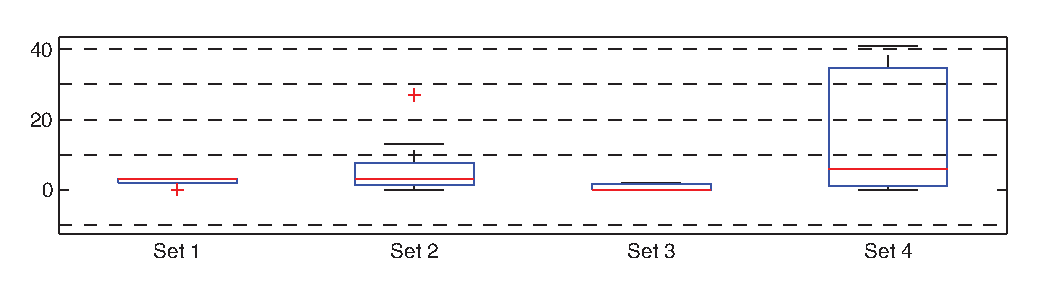
\includegraphics[width=1\textwidth]{./Figures/chapter5/boxplot_results_artificial_sets.eps}
  \caption[Box plot results artificial data sets]{Box plot of the results for the artificial data sets, indicating the number of data points difference between the actual and detected change points.}
  \label{fig:boxplot_artificial_sets}
\end{figure}

\begin{figure}
\centering
  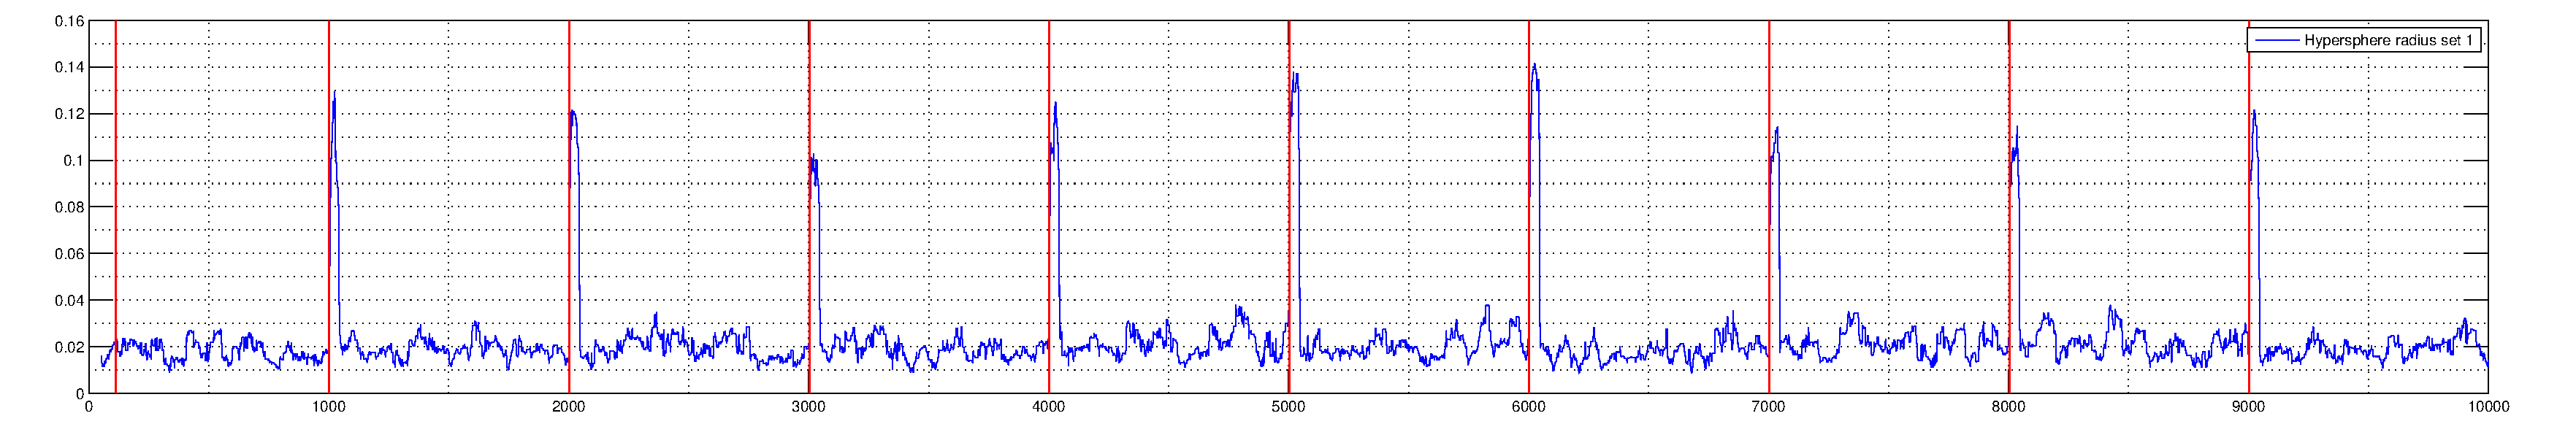
\includegraphics[width=1\textwidth]{./Figures/chapter5/set_1_results.eps}
  \caption[Fixed increasing mean, thresholds]{Hypersphere radius sizes for the \emph{Fixed increasing mean} data set with detected change points as red vertical bars.}
  \label{fig:camci_fixed_increasing_mean_thresholds}
\end{figure}

\begin{figure}
\centering
  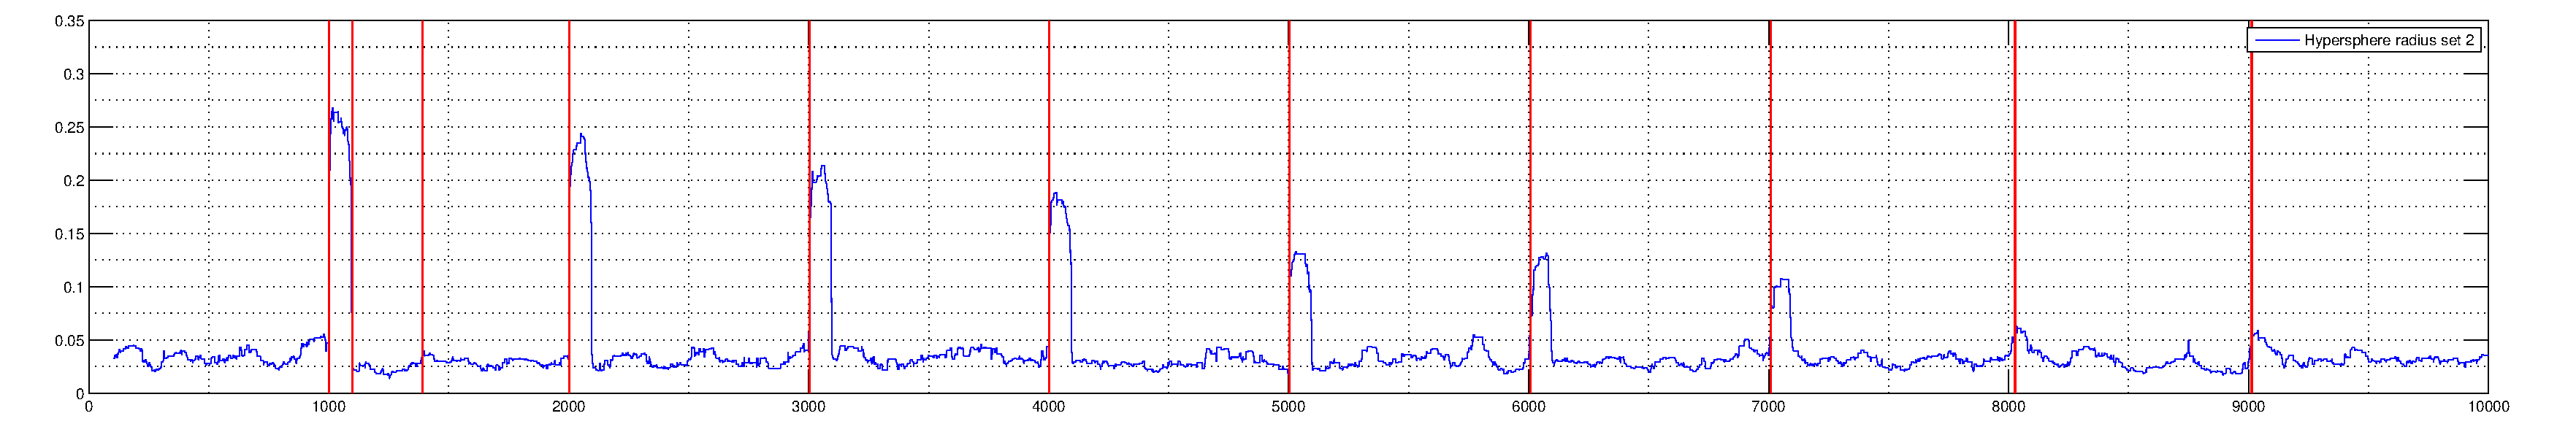
\includegraphics[width=1\textwidth]{./Figures/chapter5/set_2_results.eps}
  \caption[Reduced increasing mean, thresholds]{Hypersphere radius sizes for the \emph{Reduced increasing mean} data set with detected change points as red vertical bars.}
  \label{fig:takeuchi_reduced_increasing_mean_thresholds}
\end{figure}

\begin{figure}
\centering
  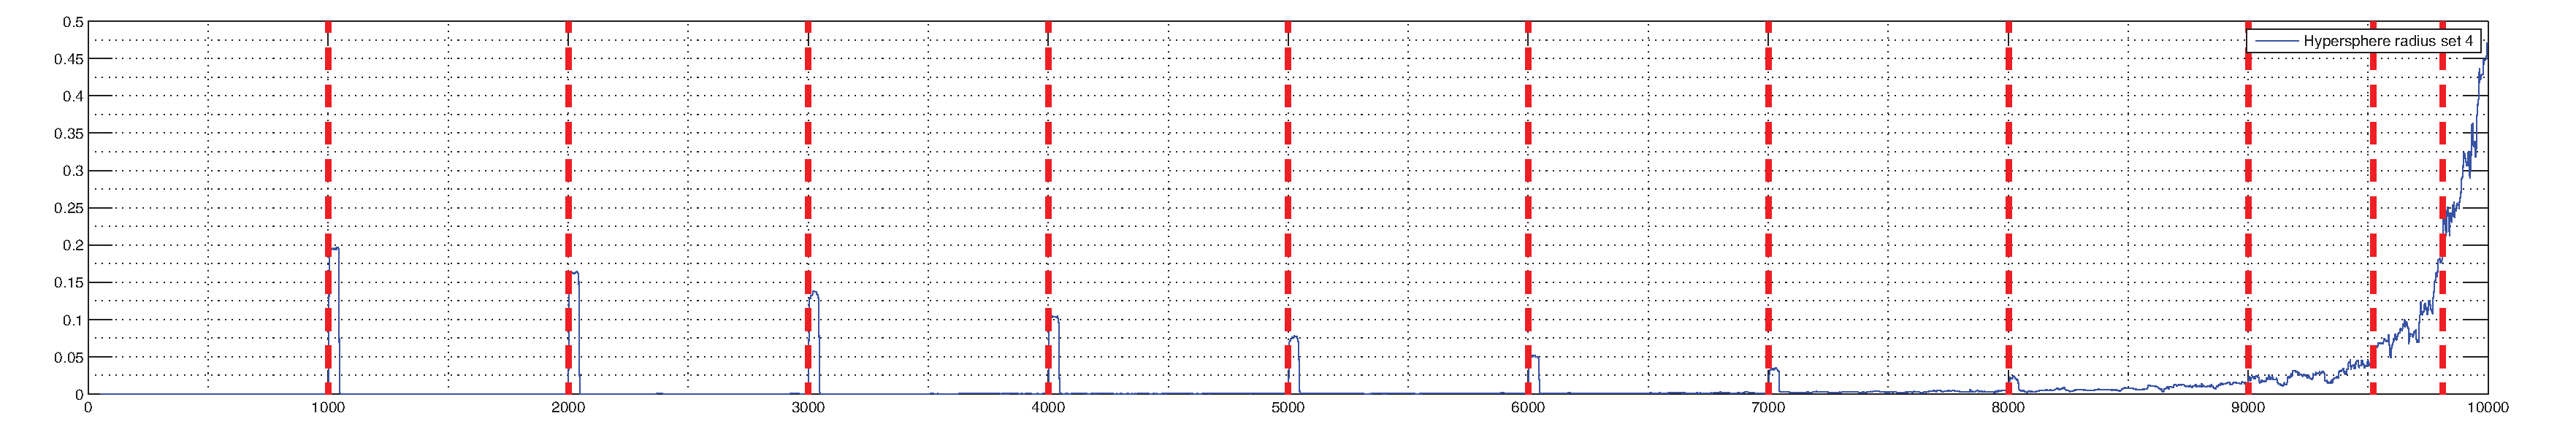
\includegraphics[width=1\textwidth]{./Figures/chapter5/set_3_results.eps}
  \caption[Reduced increasing mean, increasing variance, thresholds]{Hypersphere radius sizes for the \emph{Reduced increasing mean, increasing variance} data set with detected change points as red vertical bars.}
  \label{fig:camci_reduced_increasing_mean_increasing_variance_thresholds}
\end{figure}

\begin{figure}
\centering
  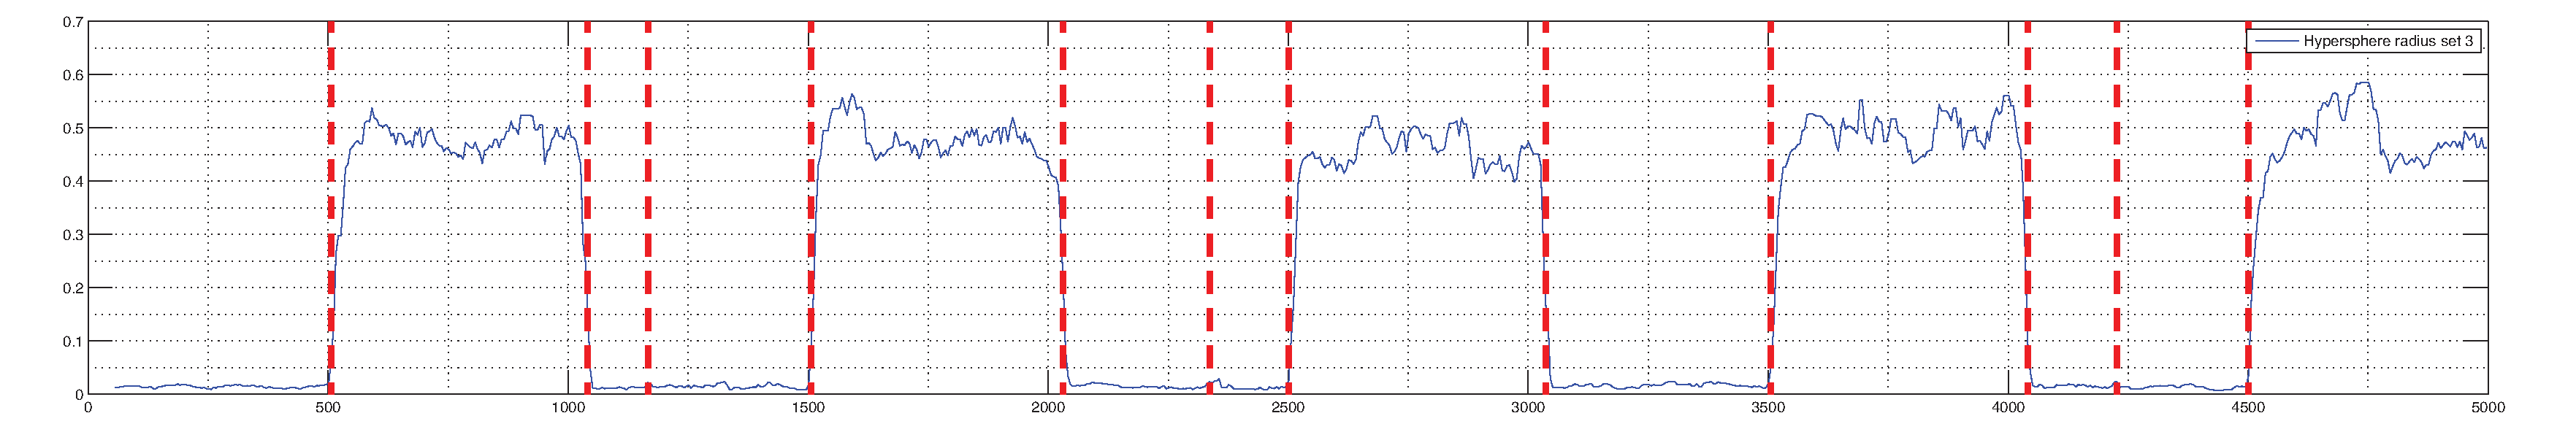
\includegraphics[width=1\textwidth]{./Figures/chapter5/set_4_results.eps}
  \caption[Alternating variance, thresholds]{Hypersphere radius sizes for the \emph{Alternating variance} data set with detected change points as red vertical bars.}
  \label{fig:camci_takeuchi_alternating_variance_thresholds}
\end{figure}